\section{Models}\label{sec:encoder}
\subsection{encoder-only model}\label{subsec:encoder-only-model}
With only-encoder, we mean that the network has only the encoder part, the decoder part is not present.

We tried to use the encoder part of the network to predict the pose of the camera, using both ResNet18 and ResNet50 as encoder.
The main different of ResNet18 and ResNet50 is the number of the output embedding, in fact, ResNet18 has output embedding dimension of 512, while ResNet50 has output embedding dimension of 2048.
We also tried with different depth of the network, in fact, we tried with \textbf{6} and \textbf{12} layers of encoder.
Then, to obtain prediction, we used a fully connected layer with 6 output neurons, one for each degree of freedom of the camera pose, we also tried an MLP that predicts the 12 numbers of the \textit{rotation matrix} and the \textit{translation vector}.

\begin{figure}[H]
    \centering
    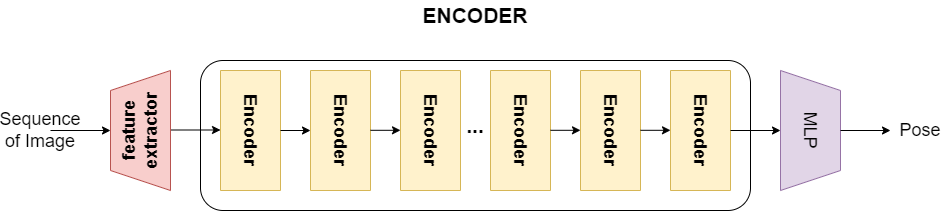
\includegraphics[width=\textwidth]{images/4_encoder_only}
    \caption{Encoder-only transformer}\label{fig:figure-encoder-only-transformer}
\end{figure}

\subsection{Encoder-decoder}\label{subsec:encoder-decoder}

For the encoder-decoder, we used the same encoder of the previous section, but we added a decoder part, which uses a vector parameter as \textit{memory} of the network.

In this version of the network, we tried the same configurations of the encoder-only model but the feature extractor ResNet50, because the network requires more memory than those available on GPU.


\begin{figure}[H]
    \centering
    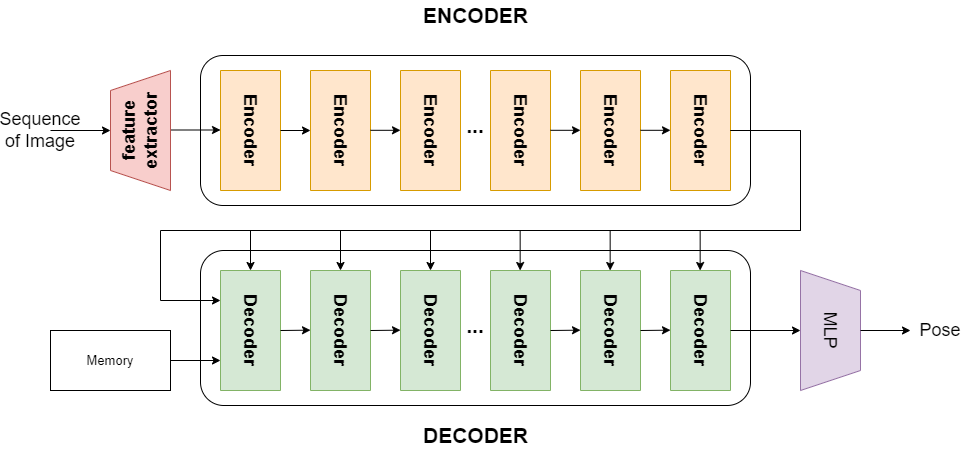
\includegraphics[width=\textwidth]{images/4_encoder_decoder}
    \caption{Encoder-Decoder transformer}\label{fig:figure-encoder-decoder-transformer}
\end{figure}

\subsection{Encoder-Decoder with Auto-encoder}\label{subsec:encoder-decoder-with-auto-encoder}
